\documentclass{article}
\usepackage[polish]{babel}
\usepackage[T1]{fontenc}
\usepackage[utf8]{inputenc}
\usepackage{graphicx}
\usepackage{float}
\usepackage[bottom=0.5cm, right=1.5cm, left=1.5cm, top=1.5cm]{geometry}
\graphicspath{{../pliki}}



\title{%
  Cyberbezpieczeństwo - laboratoria 4 \\
  \large Asymetryczne algorytmy szyfrowania}
\author{Patryk Łuszczek 272707}
\date{\today}
\begin{document}
\maketitle
\newpage
\tableofcontents
\newpage

\section{Własności algorytmów asymetrycznych}
\subsection{Zadanie 1.1}
\subsection{Zadanie 1.2}
\subsection{Zadanie 1.3 - entropia dla różnych długości klucza}

\begin{table}[H]
    \centering
    \caption{Porównanie entropii TJ dla różnych długości klucza}
    \begin{tabular}{|c|c|c|c|c|}
        \hline
        \textbf{Tekst/Klucz}         & \textbf{TJ} & \textbf{RSA512} & \textbf{RSA1024} & \textbf{RSA2048} \\ \hline
        \textbf{Jednolity}           & 0.01        & 6.22            & 7.09             & 7.48             \\ \hline
        \textbf{Średnio zróżnicoway} & 4.02        & 7.83            & 7.80             & 7.81             \\ \hline
        \textbf{Zróżnicowany}        & 4.11        & 7.81            & 7.85             & 7.85             \\ \hline
    \end{tabular}
\end{table}

\begin{figure}[H]
    \centering
    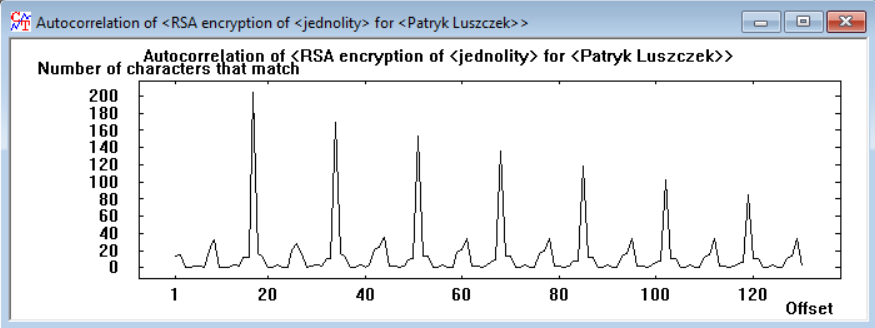
\includegraphics[width=0.8\textwidth]{korelacja_jednorodny_512.png}
    \caption{Korelacja dla tekstu jednorodnego i klucza 512bit}
\end{figure}


\begin{figure}[H]
    \centering
    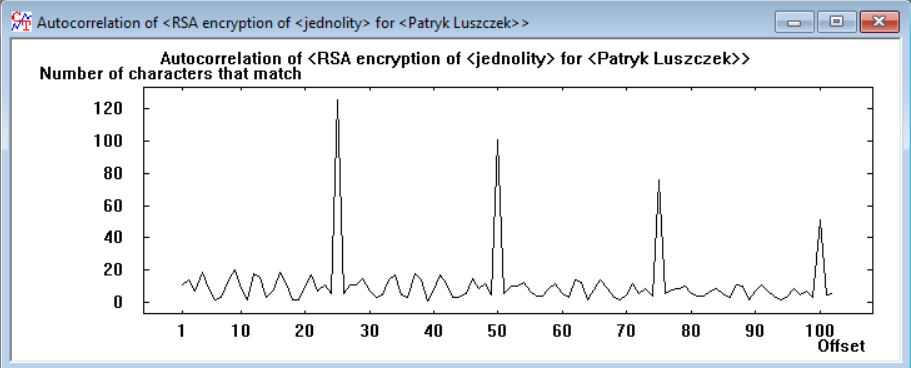
\includegraphics[width=0.8\textwidth]{korelacja_jednorodny_1024.png}
    \caption{Korelacja dla tekstu jednorodnego i klucza 1024bit}
\end{figure}



\begin{figure}[H]
    \centering
    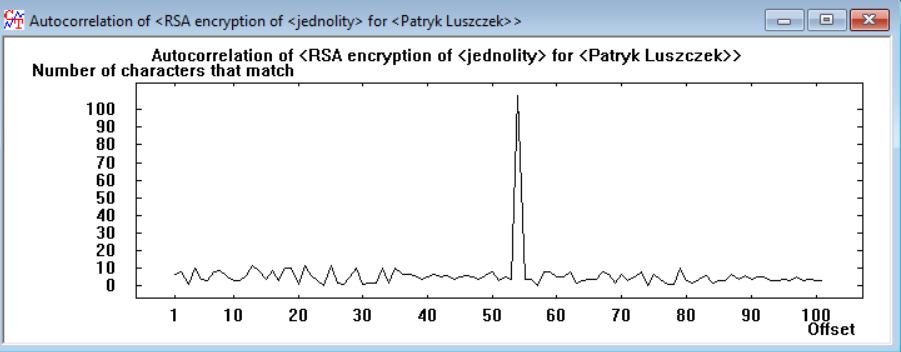
\includegraphics[width=0.8\textwidth]{korelacja_jednorodny_2048.png}
    \caption{Korelacja dla tekstu jednorodnego i klucza 2048bit}
\end{figure}


\begin{figure}[H]
    \centering
    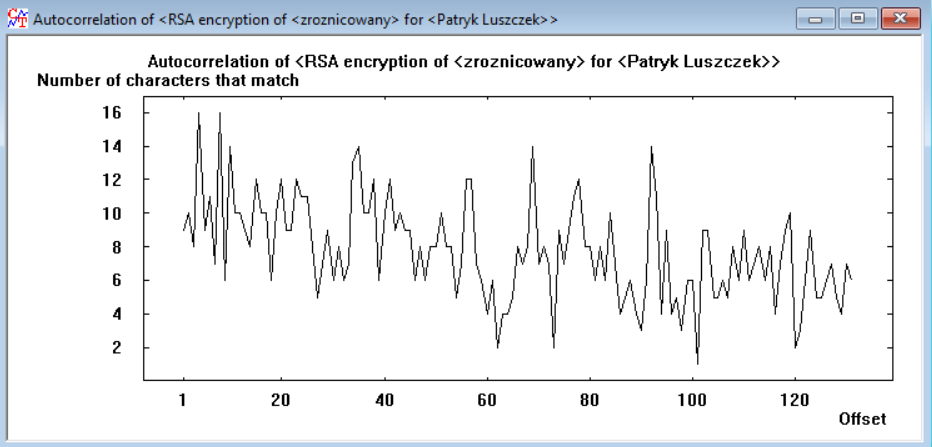
\includegraphics[width=0.8\textwidth]{korelacja_zroznicowany_512.png}
    \caption{Korelacja dla tekstu zróżnicowanego i klucza 512bit}
\end{figure}

\begin{figure}[H]
    \centering
    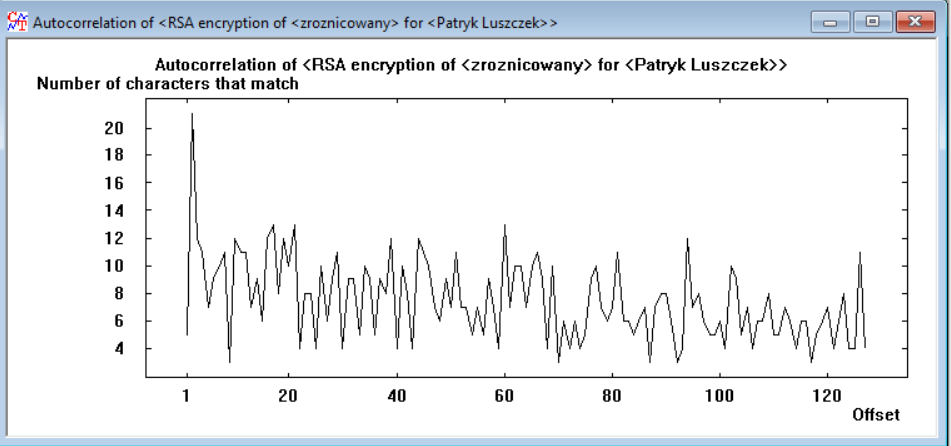
\includegraphics[width=0.8\textwidth]{korelacja_zroznicowany_2048.png}
    \caption{Korelacja dla tekstu zróżnicowanego i klucza 2048bit}
\end{figure}

\subsection{Zadanie 1.4 - czas szyfrowania RSA}

\begin{table}[H]
    \centering
    \caption{Porównanie czasu szyfrowania/deszyfrowania dla różnych długości klucza RSA i rozmiaru pliku}
    \begin{tabular}{|c|c|c|c|}
        \hline
        \textbf{Rozmiar/Klucz} & \textbf{RSA512} & \textbf{RSA1024} & \textbf{RSA2048} \\ \hline
        \textbf{1MB}           & 0.2s (4.1s)     & 0.3s (9.8s)      & 0.3s (34.2s)     \\ \hline
        \textbf{3MB}           & 0.7s (12.3s)    & 1.0s (29.3s)     & 1.9s (102.5s)    \\ \hline
        \textbf{5MB}           & 1.1s (20.9s)    & 1.7s (49.0s)     & 3.1s (170.2s)    \\ \hline
        \textbf{10MB}          & 2.2s            & 3.4s             & 6.3s             \\ \hline
        \textbf{30MB}          & 6.3s            & 10.0s            & 19.0             \\ \hline
    \end{tabular}
\end{table}

\subsection{Zadanie 1.5 - czas szyfrowania AES}

\begin{table}[H]
    \centering
    \caption{Porównanie czasu szyfrowania dla różnych długości klucza AES i rozmiaru pliku}
    \begin{tabular}{|c|c|c|c|}
        \hline
        \textbf{Rozmiar/Klucz} & \textbf{AES128} & \textbf{AES192} & \textbf{AES256} \\ \hline
        \textbf{1MB}           & natychmiast     & natychmiast     & natychmiast     \\ \hline
        \textbf{3MB}           & natychmiast     & natychmiast     & natychmiast     \\ \hline
        \textbf{5MB}           & natychmiast     & natychmiast     & natychmiast     \\ \hline
        \textbf{10MB}          & ok 0.5s         & ok 0.5s         & ok 0.5s         \\ \hline
    \end{tabular}
\end{table}



\subsection{Zadanie 1.6 - zmiany bitów w szyfrogramie}
Do eksperementu został wykorzystany tekst o wysokim stopniu zróżnicowania
\subsubsection{RSA512}
\begin{figure}[H]
    \centering
    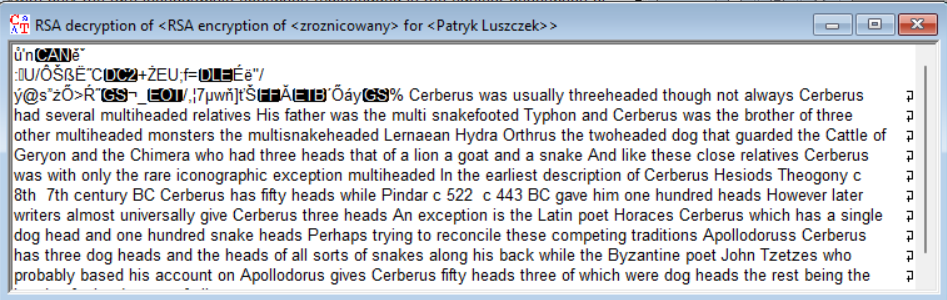
\includegraphics[width=0.8\textwidth]{zmiana_512.png}
    \caption{Wynik zmiany jednego bitu}
\end{figure}
\begin{figure}[H]
    \centering
    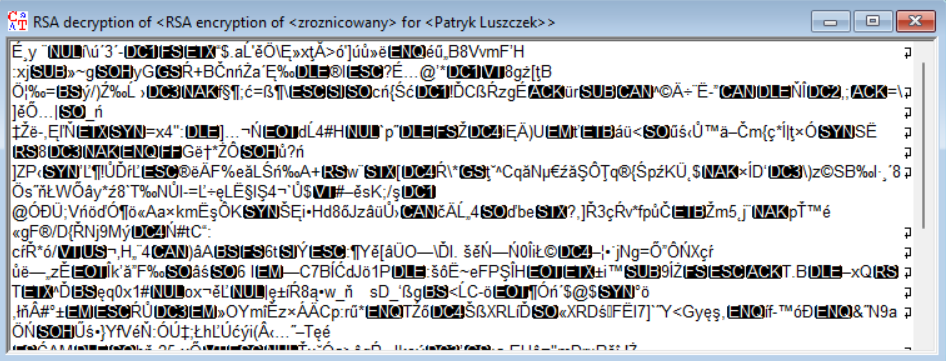
\includegraphics[width=0.8\textwidth]{usun1_512.png}
    \caption{Wynik usunięcia jednego bitu}
\end{figure}
\begin{figure}[H]
    \centering
    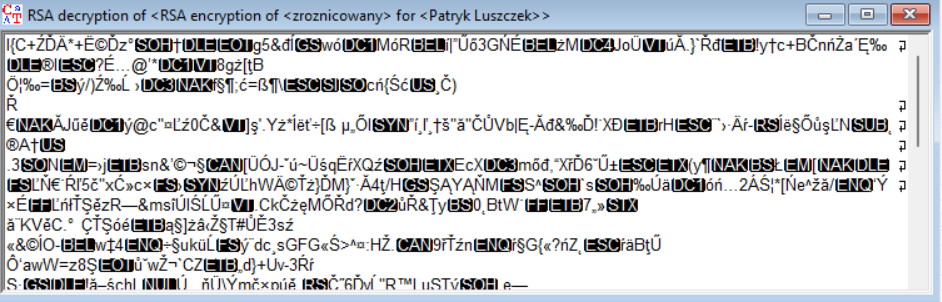
\includegraphics[width=0.8\textwidth]{usunkilka_512.png}
    \caption{Wynik usunięcia kilku bitów}
\end{figure}
\begin{figure}[H]
    \centering
    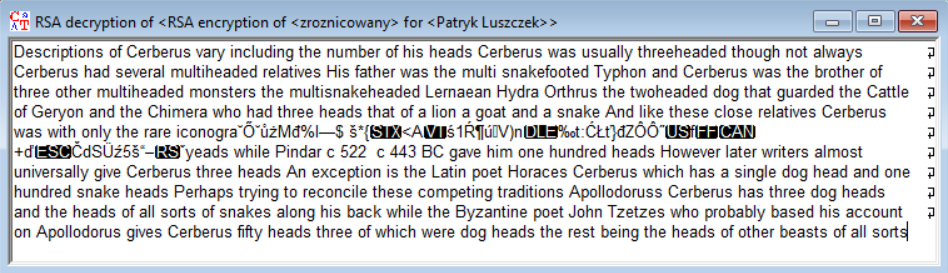
\includegraphics[width=0.8\textwidth]{usunklucz_512.png}
    \caption{Wynik usunięcia liczby bitów równych długości klucza}
\end{figure}
\subsubsection{RSA1024}
\begin{figure}[H]
    \centering
    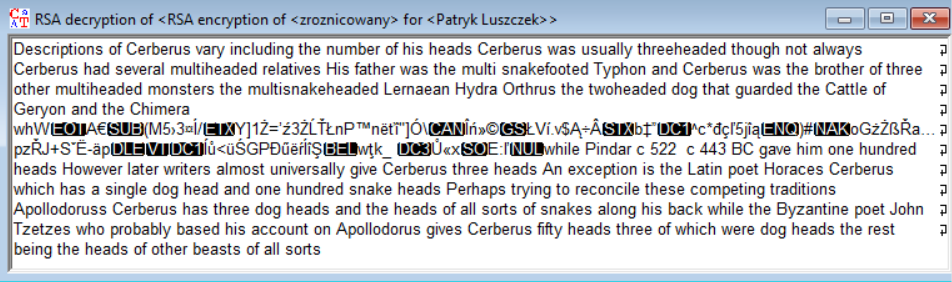
\includegraphics[width=0.8\textwidth]{usunklucz_1024.png}
    \caption{Wynik usunięcia liczby bitów równych długości klucza}
\end{figure}
\subsubsection{RSA2048}
\begin{figure}[H]
    \centering
    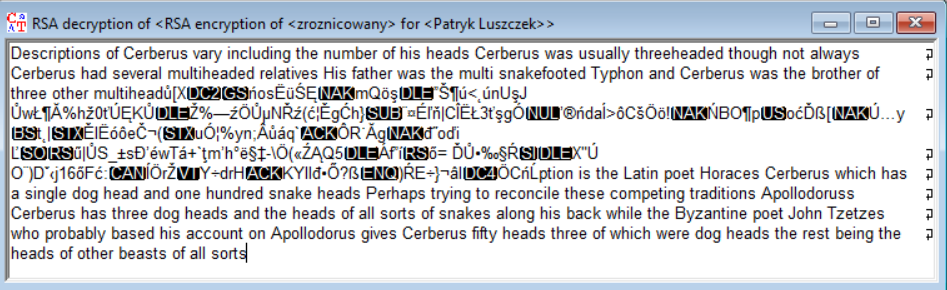
\includegraphics[width=0.8\textwidth]{usunklucz_2048.png}
    \caption{Wynik usunięcia liczby bitów równych długości klucza}
\end{figure}
\subsection*{Wnioski}
W przypadku zmiany jednego bajtu w szyfrogramie, tekst został odszyfrowany w większości poprawnie. Błędy pojawiały się w obrębie zmienianego bajtu - bloku w którym ten bajt się zawierał.
W związku z tym, ten blok stawał się nieczytelny, a jego długość zależy od długości klucza algorytmu. Dla algorytmu RSA wykorzystującego klucz 512 bitowy, blok 64 znaków stawał się nieczytelny, analogicznie dla kluczy 1024 i 2048 bitowych.
Usunięcie jednego lub kilku bajtów w szyfrogramie powodowało całkowitą korupcję tekstu. W przypadku usunięcia liczby bajtów równych długości klucza, fragment tekstu równy długości klucza stawał się nieczytelny, a reszta tekstu była odszyfrowywana poprawnie.
\subsection{Pytanie 1.7 - klucz a entropia} \label{section:pytanie 1.7}
\textbf{Treść: } Czy i jak długość klucza wpływa na entropię TT?? \\\\
Długość klucza wpływa na entropię szyfrogramu, jednak nie w jednakowy sposób - jest to zależne od entropii tekstu jawnego.
Jeśli tekst jawny był jednolity, o bardzo niskiej entropii (np. powtarzający się jeden znak), to wtedy faktycznie zwiększenie rozmiaru klucza
przynosiło efekt w postaci zwiększania się entropii TT. Jeśli natomiast tekst jawny posiadał wysoką entropię (dla eksperymentu powyżej 4.0, gdzie 4.7 to wartość maksymalna),
to zwiększanie długości klucza nie przyczyniało się do znaczącej zmiany entropii szyfrogramu - była zawse wysoka, w granicach 7.80-7.85.
\subsection{Pytanie 1.8 - klucz a korelacja}
\textbf{Treść: } Czy i jak długość klucza wpływa na korelację TT?\\\\
Długość klucza wpływa na korelację szyfrogramu, jednakże jest to zauważalne jedynie w przypadku tekstu o niskiej entropii.
Można zauważyć cykliczność w korelacji szyfrogramu, która jest zależna od długości klucza - im krótszy klucz tym częściej występują "piki" w korelacji.
\subsection{Pytanie 1.9 - entropia TT a TJ}
\textbf{Treść: } Czy i jak obserwowana entropia TT zależy od entropii TJ? \\\\
Obserwowana entropia TT jest zależna od entropii TJ, jak już wcześniej było wspomniane to w pytaniu \ref{section:pytanie 1.7}.
\subsection{Pytanie 1.10 - czas szyfrowania/deszyfrowania}
\textbf{Treść: } Jak kształtuje się czas szyfrowania/deszyfrowania w zależności od długości pliku.\\\\
Czas szyfrowania oraz deszyfrowania jest ściśle powiązany z długością pliku. Można zaobserwować niemalże liniową zależność między rozmiarem pliku, a czasem szyfrowania oraz deszfyrowania.
Plik o rozmiarze 1MB został odszyfrowany prawie natychmiastowo - narzędzie liczenia czasu w Cryptool wskazało wartość około 0.2s. Z kolei plik 5 razy większy został zaszyfrowany w około 1.1s, a plik o rozmiarze 10MB w około 2.2s.
Taką samą zależność można znaleźć w czasach deszyfrowania, gdzie najmniejszy plik został odszyfrowany w około 4.1s, a plik o rozmiarze 3MB w ok. 12.3 sekundy.
\subsection{Pytanie 1.11 - czas szyfrowania w porównaniu do algorytmów symetrycznych}
\textbf{Treść: } Jak wygląda czas operacji szyfrowania/deszyfrowania algorytmem asymetrycznym w porównaniu do realizacji tych operacji algorytmem symetrycznym. \\\\
W przeciwieństwie do algorytmów asymetrycznych, gdzie czas szyfrowania oraz deszyfrowania jest zauważalny, to w przypadku algorytmów symetrycznych te operacje były wykonywane niemalże natychmiastowo.
Oznacza to, że w celu zaszyfrowania czy zaszyfrowania algorytmem asymetrycznym musi zostać wykonane o wiele więcej, bardziej skomplikowanych operacji, co wydłuża czas działania algorytmu.
\subsection{Pytanie 1.12 - przekłamania bitów}
\textbf{Treść: } Jak wyglądają zmiany w TJ przy prowadzeniu przekłamań do TT? Jaka jest ich skala? Od czego zależy? \\\\
Wprowadzenie przykłamań do tekstu zaszyfrowanego prowadzi do utracenia części lub całej informacji. Jeśli został przekłamany jeden lub kilka bitów, to tekst po odszyfrowaniu był w większości czyelny,
a nieczytelne były fragmenty tekstu, z którego składał się blok szyfrogramu. Długość niepoprawnie odszyfrowanych fragmentów była powiązana z długościa użytego klucza. Jeśli został usunięty jeden, lub kilka bitów
to cały tekst stawał się nieczytelne. Natomiast jeśli liczba usuniętych bitów odpowiadała długości klucza szyfrogramu, to nieczytelny stawał się tylko fragment tekstu.
\subsection{Pytanie 1.13 - usunięcie fragmentu z TT}
\textbf{Treść: } Czy można usunąć fragment z TT tak, aby pozostały tekst TJ po odszyfrowaniu był czytelny? \\\\
Aby tekst po odszyfrowaniu był czytelny, to musi zostać usunięty fragment szyfrogramu o długości równej długości klucza lub jego wielokrotności. Jednakże, tekst nie będzie w pełni czytelny,
a jedynie fragmenty w których nie zostały usunięte bity w bloku.
\subsection{Pytanie 1.14 - wady i zalety}
\textbf{Treść: } Jakie są wady i zalety algorytmów asymetrycznych w porównaniu do algorytmów symetrycznych? \\\\
Ważną zaletą stosowania algorytmów asymetrycznych jest ich większe bezpieczeństwo względem algorytmów symetrycznych dzięki zastosowaniu oddzielnych kluczy używanych do szyfrowania i deszyfrowania.
Dzięki temu, odkrycie jednego klucza nie gwarantuje odnalezienia drugiego, więc znając klucz szyfrowania nie jesteśmy w stanie automatycznie go zastosować do odszyfrowania wiadomości, tak jak ma to miejsce w algorytmach symetrycznych.
Wadą jest czas potrzebny do wykonania operacji szyfrowania i deszyfrowania. W przypadku plików o dużym rozmiarze, algorytmy asymetryczne potrzebują bardzo dużo czasu do wykonania tych operacji, podczas gdy algorytmy symetryczne wykonują te operacje bardzo szybko.
Kolejnym aspektem różniącym algorytmy symetryczne od asymetrycznych jest wrażliwość na przekłamania szyfrogramu. Skala "korupcji" tekstu odszyforwanego, w przypadku błędów szyfrogramu jest o wiele większa dla algorytmów asymetrycznych niż symetrycznych.
\subsection{Pytanie 1.15 - zastosowania algorytmów}
\textbf{Treść: } W jakich zastosowaniach lepiej korzystać z algorytmów asymetrycznych, a wjakich z algorytmów symetrycznych? \\\\
Algorytmy symetryczne lepiej radzą sobie z szyfrowaniem/deszyfrowaniem dużej ilości danych, więc jeśli zależy nam na szybkim wykonaniu tych operacji, to lepiej zastosować algorytm symetryczny. Również, jeśli wiemy, że szyfrogram może ulec zakłóceniom podczas transmiji, lepiej wykorzystać algorytm symetryczny,
ponieważ jest większa szansa na to, że tekst będzie, chociażby częściowo, czytelny. Jeśli natomiast zależy nam na większym bezpieczeństwie danych, lepiej wykorzystać algorytm asymetryczny.
\end{document}
